\begin{figure}[htbp]
\centering
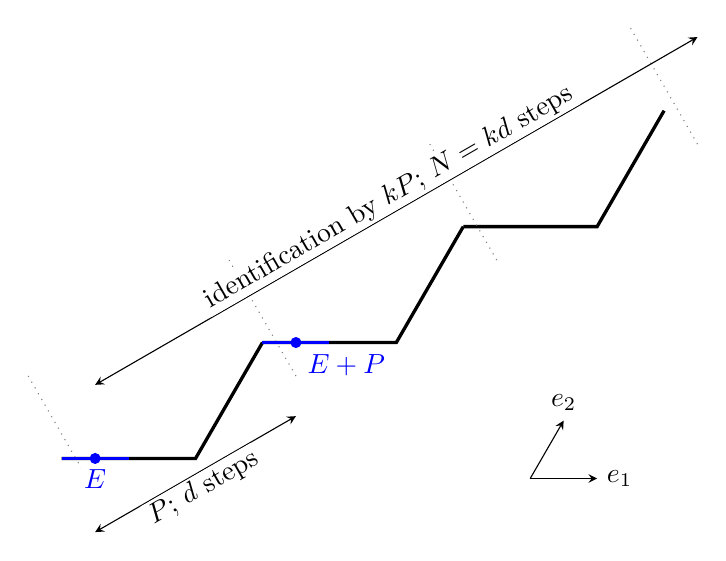
\begin{tikzpicture}[x=0.85cm,y=0.85cm,>=stealth]
  \foreach \j in {0,1,2} {
    \draw[very thick] ({3*\j},{1.73205*\j})
      -- ({3*\j+2},{1.73205*\j})
      -- ({3*\j+3},{1.73205*\j+1.73205});
    \draw[gray,dotted] ({3*\j+0.5},{1.73205*\j-0.5})
      -- ({3*\j-0.5},{1.73205*\j+1.23205});
  }
  \draw[gray,dotted] (9.5,4.69615)--(8.5,6.42820);
  \draw[very thick,blue] (0,0)--(1,0);
  \draw[very thick,blue] (3,1.73205)--(4,1.73205);
  \fill[blue] (0.5,0) circle (2pt) node[below=3pt,fill=white,inner sep=1pt] {$E$};
  \fill[blue] (3.5,1.73205) circle (2pt) node[below right=3pt,fill=white,inner sep=1pt] {$E+P$};
  \draw[<->] (0.5,-1.1)--(3.5,0.63205)
      node[midway,below,sloped,fill=white,inner sep=1pt] {$P$; $d$ steps};
  \draw[<->] (0.5,1.1)--(9.5,6.29615)
      node[midway,above,sloped,fill=white,inner sep=1pt] {identification by $kP$; $N=kd$ steps};
  \draw[->] (7,-0.3)--(8,-0.3) node[right] {$e_1$};
  \draw[->] (7,-0.3)--(7.5,0.56603) node[above] {$e_2$};
\end{tikzpicture}
\caption{A monotone staircase carrying the two identical translated marks.
The example has $P_1=P_2=2$ and $k=3$.  Translating the staircase in the
third edge direction produces the lozenge rows; the dotted segments
indicate that transverse direction.  The two background lists have
lengths $d$ and $N-d$ after adjoining one marked site to each.}
\label{u:staircase-figure}
\end{figure}
